\documentclass[authoryear]{elsarticle}
\usepackage{mathtools,upref,siunitx,upquote,fancyvrb,bbm,xspace,color,amsmath,amssymb, bm}
\usepackage[hyphens]{url}
\usepackage[utf8]{inputenc}
\usepackage{esdiff}
\usepackage{graphicx}
\usepackage{xcolor}

\DeclareSymbolFont{GreekLetters}{OML}{cmr}{m}{it} %Provide missing letters
\DeclareSymbolFont{UpSfGreekLetters}{U}{cmss}{m}{n} %Provide missing letters
\DeclareMathSymbol{\varrho}{\mathalpha}{GreekLetters}{"25}
\DeclareMathSymbol{\UpSfLambda}{\mathalpha}{UpSfGreekLetters}{"03}
\DeclareMathSymbol{\UpSfSigma}{\mathalpha}{UpSfGreekLetters}{"06}
%\newcommand{\bvec}[1]{\boldsymbol{#1}}
\providecommand{\mathbold}{\boldsymbol}
\newcommand{\bvec}[1]{\mathbold{#1}}
%\newcommand{\bvec}[1]{\text{\boldmath$#1$}}
\newcommand{\avec}[1]{\vec{#1}}
%\renewcommand{\vec}[1] {\text{\boldmath$#1$}}
%\renewcommand{\vec}[1]{\ensuremath{\mathbf{#1}}}
%\newcommand{\vecsym}[1]{\ensuremath{\boldsymbol{#1}}}
\newcommand{\vecsym}[1]{\ensuremath{\mathbold{#1}}}
\def\bbl{\text{\boldmath$\{$}}
\def\bbr{\text{\boldmath$\}$}}
\newcommand{\bbrace}[1]{\bbl #1 \bbr}
\newcommand{\bbbrace}[1]{\mathopen{\pmb{\bigg\{}}#1\mathclose{\pmb{\bigg\}}}}
\def\betahat{\hat\beta}
\newcommand{\dif}{{\rm d}}

\newlength{\overwdth}
\def\overstrike#1{ 
\settowidth{\overwdth}{#1}\makebox[0pt][l]{\rule[0.5ex]{\overwdth}{0.1ex}}#1}

\makeatletter
\newcommand*\bigcdot{\mathpalette\bigcdot@{.7}}
\newcommand*\bigcdot@[2]{\mathbin{\vcenter{\hbox{\scalebox{#2}{$\m@th#1\bullet$}}}}}
\makeatother

\def\abs#1{\ensuremath{\left \lvert #1 \right \rvert}}
\newcommand{\normabs}[1]{\ensuremath{\lvert #1 \rvert}}
\newcommand{\bigabs}[1]{\ensuremath{\bigl \lvert #1 \bigr \rvert}}
\newcommand{\Bigabs}[1]{\ensuremath{\Bigl \lvert #1 \Bigr \rvert}}
\newcommand{\biggabs}[1]{\ensuremath{\biggl \lvert #1 \biggr \rvert}}
\newcommand{\Biggabs}[1]{\ensuremath{\Biggl \lvert #1 \Biggr \rvert}}
\newcommand{\norm}[2][{}]{\ensuremath{\left \lVert #2 \right \rVert}_{#1}}
\newcommand{\normnorm}[2][{}]{\ensuremath{\lVert #2 \rVert}_{#1}}
\newcommand{\bignorm}[2][{}]{\ensuremath{\bigl \lVert #2 \bigr \rVert}_{#1}}
\newcommand{\Bignorm}[2][{}]{\ensuremath{\Bigl \lVert #2 \Bigr \rVert}_{#1}}
\newcommand{\biggnorm}[2][{}]{\ensuremath{\biggl \lVert #2 \biggr \rVert}_{#1}}
\newcommand{\Biggnorm}[2][{}]{\ensuremath{\Biggl \lVert #2 \Biggr \rVert}_{#1}}
\newcommand{\ip}[3][{}]{\ensuremath{\left \langle #2, #3 \right \rangle_{#1}}}

\newcommand{\bigvecpar}[3]{\ensuremath{\bigl ( #1 \bigr )_{#2}^{#3}}}
\newcommand{\Bigvecpar}[3]{\ensuremath{\Bigl ( #1 \Bigr )_{#2}^{#3}}}
\newcommand{\biggvecpar}[3]{\ensuremath{\biggl ( #1 \biggr )_{#2}^{#3}}}
\newcommand{\bigpar}[1]{\ensuremath{\bigl ( #1 \bigr )}}
\newcommand{\Bigpar}[1]{\ensuremath{\Bigl ( #1 \Bigr )}}
\newcommand{\biggpar}[1]{\ensuremath{\biggl ( #1 \biggr )}}

\newcommand{\IIDsim}{\overset{\textup{IID}}{\sim}}
\newcommand{\LDsim}{\overset{\textup{LD}}{\sim}}

\DeclareMathOperator{\success}{succ}
\DeclareMathOperator{\sinc}{sinc}
\DeclareMathOperator{\sech}{sech}
\DeclareMathOperator{\csch}{csch}
\DeclareMathOperator{\dist}{dist}
\DeclareMathOperator{\spn}{span}
\DeclareMathOperator{\sgn}{sgn}
\DeclareMathOperator*{\rmse}{rmse}
\DeclareMathOperator{\Prob}{\mathbb{P}}
\DeclareMathOperator{\Ex}{\mathbb{E}}
\DeclareMathOperator{\rank}{rank}
\DeclareMathOperator{\erfc}{erfc}
\DeclareMathOperator{\erf}{erf}
\DeclareMathOperator{\cov}{cov}
\DeclareMathOperator{\cost}{cost}
\DeclareMathOperator{\comp}{comp}
\DeclareMathOperator{\corr}{corr}
\DeclareMathOperator{\diag}{diag}
\DeclareMathOperator{\var}{var}
\DeclareMathOperator{\opt}{opt}
\DeclareMathOperator{\brandnew}{new}
\DeclareMathOperator{\std}{std}
\DeclareMathOperator{\kurt}{kurt}
\DeclareMathOperator{\med}{med}
\DeclareMathOperator{\vol}{vol}
\DeclareMathOperator{\bias}{bias}
\DeclareMathOperator*{\argmax}{argmax}
\DeclareMathOperator*{\argmin}{argmin}
\DeclareMathOperator{\sign}{sign}
\DeclareMathOperator{\spann}{span}
\DeclareMathOperator{\cond}{cond}
\DeclareMathOperator{\trace}{trace}
\DeclareMathOperator{\Si}{Si}
%\DeclareMathOperator{\diag}{diag}
\DeclareMathOperator{\col}{col}
\DeclareMathOperator{\nullspace}{null}
\DeclareMathOperator{\Order}{{\mathcal O}}
%\DeclareMathOperator{\rank}{rank}

\newcommand{\vzero}{\bvec{0}}
\newcommand{\vone}{\bvec{1}}
\newcommand{\vinf}{\bvec{\infty}}
\newcommand{\va}{\bvec{a}}
\newcommand{\vA}{\bvec{A}}
\newcommand{\vb}{\bvec{b}}
\newcommand{\vB}{\bvec{B}}
\newcommand{\vc}{\bvec{c}}
\newcommand{\vC}{\bvec{C}}
\newcommand{\vd}{\bvec{d}}
\newcommand{\vD}{\bvec{D}}
\newcommand{\ve}{\bvec{e}}
\newcommand{\vf}{\bvec{f}}
\newcommand{\vF}{\bvec{F}}
\newcommand{\vg}{\bvec{g}}
\newcommand{\vG}{\bvec{G}}
\newcommand{\vh}{\bvec{h}}
\newcommand{\vi}{\bvec{i}}
\newcommand{\vj}{\bvec{j}}
\newcommand{\vk}{\bvec{k}}
\newcommand{\vK}{\bvec{K}}
\newcommand{\vl}{\bvec{l}}
\newcommand{\vell}{\bvec{\ell}}
\newcommand{\vL}{\bvec{L}}
\newcommand{\vm}{\bvec{m}}
\newcommand{\vp}{\bvec{p}}
\newcommand{\vq}{\bvec{q}}
\newcommand{\vr}{\bvec{r}}
\newcommand{\vs}{\bvec{s}}
\newcommand{\vS}{\bvec{S}}
\newcommand{\vt}{\bvec{t}}
\newcommand{\vT}{\bvec{T}}
\newcommand{\vu}{\bvec{u}}
\newcommand{\vU}{\bvec{U}}
\newcommand{\vv}{\bvec{v}}
\newcommand{\vV}{\bvec{V}}
\newcommand{\vw}{\bvec{w}}
\newcommand{\vW}{\bvec{W}}
\newcommand{\vx}{\bvec{x}}
\newcommand{\vX}{\bvec{X}}
\newcommand{\vy}{\bvec{y}}
\newcommand{\vY}{\bvec{Y}}
\newcommand{\vz}{\bvec{z}}
\newcommand{\vZ}{\bvec{Z}}

\newcommand{\ai}{\avec{\imath}}
\newcommand{\ak}{\avec{k}}
\newcommand{\avi}{\avec{\bvec{\imath}}}
\newcommand{\at}{\avec{t}}
\newcommand{\avt}{\avec{\vt}}
\newcommand{\ax}{\avec{x}}
\newcommand{\ah}{\avec{h}}
\newcommand{\akappa}{\avec{\kappa}}
\newcommand{\avx}{\avec{\vx}}
\newcommand{\ay}{\avec{y}}
\newcommand{\avy}{\avec{\vy}}
\newcommand{\avz}{\avec{\vz}}
\newcommand{\avzero}{\avec{\vzero}}
\newcommand{\aomega}{\avec{\omega}}
\newcommand{\avomega}{\avec{\vomega}}
\newcommand{\anu}{\avec{\nu}}
\newcommand{\avnu}{\avec{\vnu}}
\newcommand{\aDelta}{\avec{\Delta}}
\newcommand{\avDelta}{\avec{\vDelta}}

\newcommand{\valpha}{\bvec{\alpha}}
\newcommand{\vbeta}{\bvec{\beta}}
\newcommand{\vgamma}{\bvec{\gamma}}
\newcommand{\vGamma}{\bvec{\Gamma}}
\newcommand{\vdelta}{\bvec{\delta}}
\newcommand{\vDelta}{\bvec{\Delta}}
\newcommand{\vphi}{\bvec{\phi}}
\newcommand{\vvphi}{\bvec{\varphi}}
\newcommand{\vPhi}{\bvec{\Phi}}
\newcommand{\vomega}{\bvec{\omega}}
\newcommand{\vkappa}{\bvec{\kappa}}
\newcommand{\vlambda}{\bvec{\lambda}}
\newcommand{\vmu}{\bvec{\mu}}
\newcommand{\vnu}{\bvec{\nu}}
\newcommand{\vpsi}{\bvec{\psi}}
\newcommand{\vPsi}{\bvec{\Psi}}
\newcommand{\vepsilon}{\bvec{\epsilon}}
\newcommand{\veps}{\bvec{\varepsilon}}
\newcommand{\veta}{\bvec{\eta}}
\newcommand{\vxi}{\bvec{\xi}}
\newcommand{\vtheta}{\bvec{\theta}}
\newcommand{\vtau}{\bvec{\tau}}
\newcommand{\vzeta}{\bvec{\zeta}}

\newcommand{\hA}{\widehat{A}}
\newcommand{\hvb}{\hat{\vb}}
\newcommand{\hcc}{\widehat{\cc}}
\newcommand{\hD}{\widehat{D}}
\newcommand{\hE}{\widehat{E}}
\newcommand{\hf}{\widehat{f}}
\newcommand{\hF}{\widehat{F}}
\newcommand{\hg}{\hat{g}}
\newcommand{\hvf}{\widehat{\bvec{f}}}
\newcommand{\hh}{\hat{h}}
\newcommand{\hH}{\widehat{H}}
\newcommand{\hi}{\hat{\imath}}
\newcommand{\hI}{\hat{I}}
\newcommand{\hci}{\widehat{\ci}}
\newcommand{\hj}{\hat{\jmath}}
\newcommand{\hJ}{\widehat{J}}
\newcommand{\hp}{\hat{p}}
\newcommand{\hP}{\widehat{P}}
\newcommand{\hS}{\widehat{S}}
\newcommand{\hv}{\hat{v}}
\newcommand{\hV}{\widehat{V}}
\newcommand{\hx}{\hat{x}}
\newcommand{\hX}{\widehat{X}}
\newcommand{\hvX}{\widehat{\vX}}
\newcommand{\hy}{\hat{y}}
\newcommand{\hvy}{\hat{\vy}}
\newcommand{\hY}{\widehat{Y}}
\newcommand{\hvY}{\widehat{\vY}}
\newcommand{\hZ}{\widehat{Z}}
\newcommand{\hvZ}{\widehat{\vZ}}

\newcommand{\halpha}{\hat{\alpha}}
\newcommand{\hvalpha}{\hat{\valpha}}
\newcommand{\hbeta}{\hat{\beta}}
\newcommand{\hvbeta}{\hat{\vbeta}}
\newcommand{\hgamma}{\hat{\gamma}}
\newcommand{\hvgamma}{\hat{\vgamma}}
\newcommand{\hdelta}{\hat{\delta}}
\newcommand{\hvareps}{\hat{\varepsilon}}
\newcommand{\hveps}{\hat{\veps}}
\newcommand{\hmu}{\hat{\mu}}
\newcommand{\hnu}{\hat{\nu}}
\newcommand{\hvnu}{\widehat{\vnu}}
\newcommand{\homega}{\widehat{\omega}}
\newcommand{\hPi}{\widehat{\Pi}}
\newcommand{\hrho}{\hat{\rho}}
\newcommand{\hsigma}{\hat{\sigma}}
\newcommand{\htheta}{\hat{\theta}}
\newcommand{\hTheta}{\hat{\Theta}}
\newcommand{\htau}{\hat{\tau}}
\newcommand{\hxi}{\hat{\xi}}
\newcommand{\hvxi}{\hat{\vxi}}

\newcommand{\otau}{\overline{\tau}}
\newcommand{\oY}{\overline{Y}}

\newcommand{\rD}{\mathring{D}}
\newcommand{\rf}{\mathring{f}}
\newcommand{\rV}{\mathring{V}}

\newcommand{\ta}{\tilde{a}}
\newcommand{\tA}{\tilde{A}}
\newcommand{\tmA}{\widetilde{\mA}}
\newcommand{\tvb}{\widetilde{\vb}}
\newcommand{\tcb}{\widetilde{\cb}}
\newcommand{\tB}{\widetilde{B}}
\newcommand{\tc}{\tilde{c}}
\newcommand{\tvc}{\tilde{\vc}}
\newcommand{\tfc}{\tilde{\fc}}
\newcommand{\tC}{\widetilde{C}}
\newcommand{\tcc}{\widetilde{\cc}}
\newcommand{\tD}{\widetilde{D}}
\newcommand{\te}{\tilde{e}}
\newcommand{\tE}{\widetilde{E}}
\newcommand{\tf}{\widetilde{f}}
\newcommand{\tF}{\widetilde{F}}
\newcommand{\tvf}{\tilde{\vf}}
\newcommand{\tcf}{\widetilde{\cf}}
\newcommand{\tg}{\tilde{g}}
\newcommand{\tvg}{\widetilde{\vg}}
\newcommand{\tG}{\widetilde{G}}
\newcommand{\tildeh}{\tilde{h}}
\newcommand{\tH}{\widetilde{H}}
\newcommand{\tch}{\widetilde{\ch}}
\newcommand{\tK}{\widetilde{K}}
\newcommand{\tvk}{\tilde{\vk}}
\newcommand{\tM}{\widetilde{M}}
\newcommand{\tn}{\tilde{n}}
\newcommand{\tN}{\widetilde{N}}
\newcommand{\tQ}{\widetilde{Q}}
\newcommand{\tR}{\widetilde{R}}
\newcommand{\tS}{\widetilde{S}}
\newcommand{\tvS}{\widetilde{\vS}}
\newcommand{\tT}{\widetilde{T}}
\newcommand{\tv}{\tilde{v}}
\newcommand{\tV}{\widetilde{V}}
\newcommand{\tvx}{\tilde{\vx}}
\newcommand{\tW}{\widetilde{W}}
\newcommand{\tx}{\tilde{x}}
\newcommand{\tX}{\widetilde{X}}
\newcommand{\tvX}{\widetilde{\vX}}
\newcommand{\ty}{\tilde{y}}
\newcommand{\tvy}{\tilde{\vy}}
\newcommand{\tz}{\tilde{z}}
\newcommand{\tZ}{\widetilde{Z}}
\newcommand{\tL}{\widetilde{L}}
\newcommand{\tP}{\widetilde{P}}
\newcommand{\tY}{\widetilde{Y}}
\newcommand{\tmH}{\widetilde{\mH}}
\newcommand{\tmK}{\widetilde{\mK}}
\newcommand{\tmM}{\widetilde{\mM}}
\newcommand{\tmQ}{\widetilde{\mQ}}
\newcommand{\tct}{\widetilde{\ct}}
\newcommand{\talpha}{\tilde{\alpha}}
\newcommand{\tdelta}{\tilde{\delta}}
\newcommand{\tDelta}{\tilde{\Delta}}
\newcommand{\tvareps}{\tilde{\varepsilon}}
\newcommand{\tveps}{\tilde{\veps}}
\newcommand{\tlambda}{\tilde{\lambda}}
\newcommand{\tmu}{\tilde{\mu}}
\newcommand{\tnu}{\tilde{\nu}}
\newcommand{\trho}{\tilde{\rho}}
\newcommand{\tvarrho}{\tilde{\varrho}}
\newcommand{\ttheta}{\tilde{\theta}}
\newcommand{\tsigma}{\tilde{\sigma}}
\newcommand{\tvmu}{\tilde{\vmu}}
\newcommand{\tphi}{\tilde{\phi}}
\newcommand{\tPhi}{\widetilde{\Phi}}
\newcommand{\tvphi}{\tilde{\vphi}}
\newcommand{\ttau}{\tilde{\tau}}
\newcommand{\txi}{\tilde{\xi}}
\newcommand{\tvxi}{\tilde{\vxi}}


\newcommand{\mA}{\mathsf{A}}
\newcommand{\mB}{\mathsf{B}}
\newcommand{\mC}{\mathsf{C}}
\newcommand{\vmC}{\bvec{\mC}}
\newcommand{\mD}{\mathsf{D}}
\newcommand{\mF}{\mathsf{F}}
\newcommand{\mG}{\mathsf{G}}
\newcommand{\mH}{\mathsf{H}}
\newcommand{\mI}{\mathsf{I}}
\newcommand{\mK}{\mathsf{K}}
\newcommand{\mL}{\mathsf{L}}
\newcommand{\mM}{\mathsf{M}}
\newcommand{\mP}{\mathsf{P}}
\newcommand{\mQ}{\mathsf{Q}}
\newcommand{\mR}{\mathsf{R}}
\newcommand{\mS}{\mathsf{S}}
\newcommand{\mT}{\mathsf{T}}
\newcommand{\mU}{\mathsf{U}}
\newcommand{\mV}{\mathsf{V}}
\newcommand{\mW}{\mathsf{W}}
\newcommand{\mX}{\mathsf{X}}
\newcommand{\mLambda}{\UpSfLambda}
\newcommand{\mSigma}{\UpSfSigma}
\newcommand{\mzero}{\mathsf{0}}
\newcommand{\mGamma}{\mathsf{\Gamma}}

\newcommand{\bbE}{\mathbb{E}}
\newcommand{\bbF}{\mathbb{F}}
\newcommand{\bbK}{\mathbb{K}}
\newcommand{\bbV}{\mathbb{V}}
\newcommand{\bbZ}{\mathbb{Z}}
\newcommand{\bbone}{\mathbbm{1}}
\newcommand{\naturals}{\mathbb{N}}
\newcommand{\reals}{\mathbb{R}}
\newcommand{\integers}{\mathbb{Z}}
\newcommand{\natzero}{\mathbb{N}_{0}}
\newcommand{\rationals}{\mathbb{Q}}
\newcommand{\complex}{\mathbb{C}}

\newcommand{\ca}{\mathcal{A}}
\newcommand{\cb}{\mathcal{B}}
\providecommand{\cc}{\mathcal{C}}
\newcommand{\cd}{\mathcal{D}}
\newcommand{\ce}{\mathcal{E}}
\newcommand{\cf}{\mathcal{F}}
\newcommand{\cg}{\mathcal{G}}
\newcommand{\ch}{\mathcal{H}}
\newcommand{\ci}{\mathcal{I}}
\newcommand{\cj}{\mathcal{J}}
\newcommand{\ck}{\mathcal{K}}
\newcommand{\cl}{\mathcal{L}}
\newcommand{\cm}{\mathcal{M}}
\newcommand{\tcm}{\widetilde{\cm}}
\newcommand{\cn}{\mathcal{N}}
\newcommand{\cp}{\mathcal{P}}
\newcommand{\calr}{\mathcal{R}}
\newcommand{\cs}{\mathcal{S}}
\newcommand{\ct}{\mathcal{T}}
\newcommand{\cu}{\mathcal{U}}
\newcommand{\cv}{\mathcal{V}}
\newcommand{\cw}{\mathcal{W}}
\newcommand{\cx}{\mathcal{X}}
\newcommand{\tcx}{\widetilde{\cx}}
\newcommand{\cy}{\mathcal{Y}}
\newcommand{\cz}{\mathcal{Z}}

\newcommand{\fc}{\mathfrak{c}}
\newcommand{\fC}{\mathfrak{C}}
\newcommand{\fh}{\mathfrak{h}}
\newcommand{\fu}{\mathfrak{u}}

\newcommand{\me}{\ensuremath{\mathrm{e}}} % for math number 'e', 2.718 281 8..., tha base of natural logarithms
\newcommand{\mi}{\ensuremath{\mathrm{i}}} % for math number 'i', the imaginary unit
\newcommand{\mpi}{\ensuremath{\mathrm{\pi}}} % for math number 'pi', the circumference of a circle of diameter 1



\usepackage{algpseudocode}
\usepackage{algorithm, algorithmicx}
\algnewcommand\algorithmicparam{\textbf{Parameters:}}
\algnewcommand\PARAM{\item[\algorithmicparam]}
\algnewcommand\algorithmicinput{\textbf{Input:}}
\algnewcommand\INPUT{\item[\algorithmicinput]}
\algnewcommand\RETURN{\State \textbf{Return }}

\newcommand{\tr}{\widetilde{r}}
\newcommand{\appxintn}{\appxint_n}
\DeclareMathOperator{\appxint}{\hat{I}}
\DeclareMathOperator{\trun}{trunc}
\newcommand{\onetos}{1\!:\!s}

\newcommand{\FredNote}[1]{{\color{blue}#1}}

\newcommand{\LarysaNote}[1]{{\color{violet}#1}}
\begin{document}

% \maketitle
\section{Introduction}



Multidimensional integrals arise in various fields and practical applications \LarysaNote{such as quantitative finance, statistics , and physics } \FredNote{Often these arise as expectations of random variables.}  However, many such integrals cannot be computed analytically and, thus, numerical methods are often utilized. \FredNote{A common approach to approximating an integral that represents a population mean is by a sample mean:} 
\[
\mathbb{E}[f(\underbrace{\vX}_{\sim \mathcal{U}[0,1]^d})] : = \int_{[0,1)^s} f(\vx) \, \dif \vx \approx \frac{1}{n} \sum_{i=0}^{n-1} f(\vz_i) =:\appxintn(f),
\]
\citep{DicEtal22a,Nie92,SloJoe94}.
The nodeset, $\{\vz_0, \vz_1, \ldots \}$, is chosen as independent and identically distributed (IID), which corresponds to simple Monte Carlo. However, the nodeset may be chosen to be more evenly distributed, which corresponds to quasi-Monte Carlo methods. Lattices are a popular choice of nodes $\{\vz_i\}_{i=0}^{\infty} \in [0,1)^s$ for such approximations. \\

% what we are doing 

\LarysaNote{In this work we establish the upper bounds on the figures of merit for extensible lattices with arbitrary cardinality $n$. }
\cite{HicNie03a} established the existence of extensible lattices with good generating vectors for the preferred values $n = b, b^2, \ldots$.  Our purpose is to extend these results to all positive $n$, recognizing that the upper bounds on the figures of merit will be somewhat worse for general $n$ than for powers of the base. \\

\LarysaNote{We consider a case of an arbitrary positive $n$ and the case of $n = \lambda b^p$, where $\lambda$ is a small odd integer. We found $P_{\alpha}$  } \\

   
In the next section, we give more background on extensible lattices. In Section 2 we go over the figures of merit and the worst case error analysis for arbitrary $n$ for integrands that have absolutely summable Fourier series. In Section 3 we derive upper bounds on the figure of merit % P_alpha 
for $n$ other than $b^m$, and in Section 4 we generalize the results to other spaces of integrands and error measures. 

\begin{figure}[h]
\centering
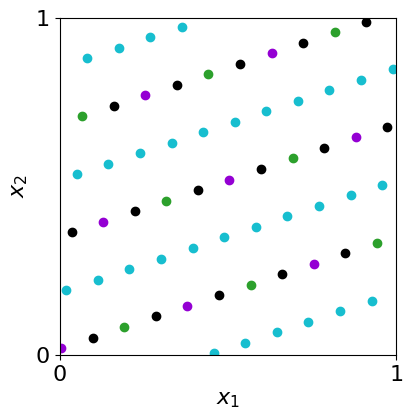
\includegraphics[width=5cm,clip]{lattice-plot.png}
\caption{Two-dimensional Shifted Lattice}
\label{fig:enter-label}
\end{figure}
\section{Background}

Historically, lattice points were initially constructed as sets with fixed cardinality, $n$, and took the form
\begin{equation} \label{eq:lat}
    \{\vz_i = i \vh/n \bmod{\vone} : i=0,1, \ldots, n-1 \} \in [0,1)^s,
\end{equation}
where $\vh \in \{1, \ldots, n-1\}^s$ is the \emph{generating vector}.  A (random) shift, $\vDelta \in [0,1)^s$, is often added:
\begin{equation} \label{eq:shlat}
    \{\vz_i = i \vh/n + \vDelta \pmod{\vone} : i=0,1, \ldots, n-1 \} \in [0,1)^s.
\end{equation}



% \cite{HicNie03a} established the existence of extensible lattices with good generating vectors for the preferred values $n = b, b^2, \ldots$.  The purpose of this thesis is to extend these results to all positive $n$, recognizing that the upper bounds on the figures of merit will be somewhat worse for general $n$ than for powers of the base. 

% In the next section, we give more background on extensible lattices. In Section 2 we go over the figures of merit and the worst case error analysis for arbitrary $n$ for integrands that have absolutely summable Fourier series. In Section 3 we derive upper bounds on the figure of merit % P_alpha 
% for $n$ other than $b^m$, and in Section 4 we generalize the results to other spaces of integrands and error measures. 














% Lattices are a popular choice of nodes $\{\vz_i\}_{i=0}^{\infty} \in [0,1)^s$ for approximating multidimensional integrals by a sample mean,
% \[
% \int_{[0,1)^s} f(\vx) \, \dif \vx \approx \frac{1}{n} \sum_{i=0}^{n-1} f(\vz_i) =:\appxintn(f),
% \]
% \citep{DicEtal22a,Nie92,SloJoe94}.



% \cite{HicNie03a} established the existence of extensible lattices with good generating vectors for the preferred values $n = b, b^2, \ldots$.  The purpose of this thesis is to extend these results to all positive $n$, recognizing that the upper bounds on the figures of merit will be somewhat worse for general $n$ than for powers of the base. 

% \begin{figure}[h]
% \centering
% 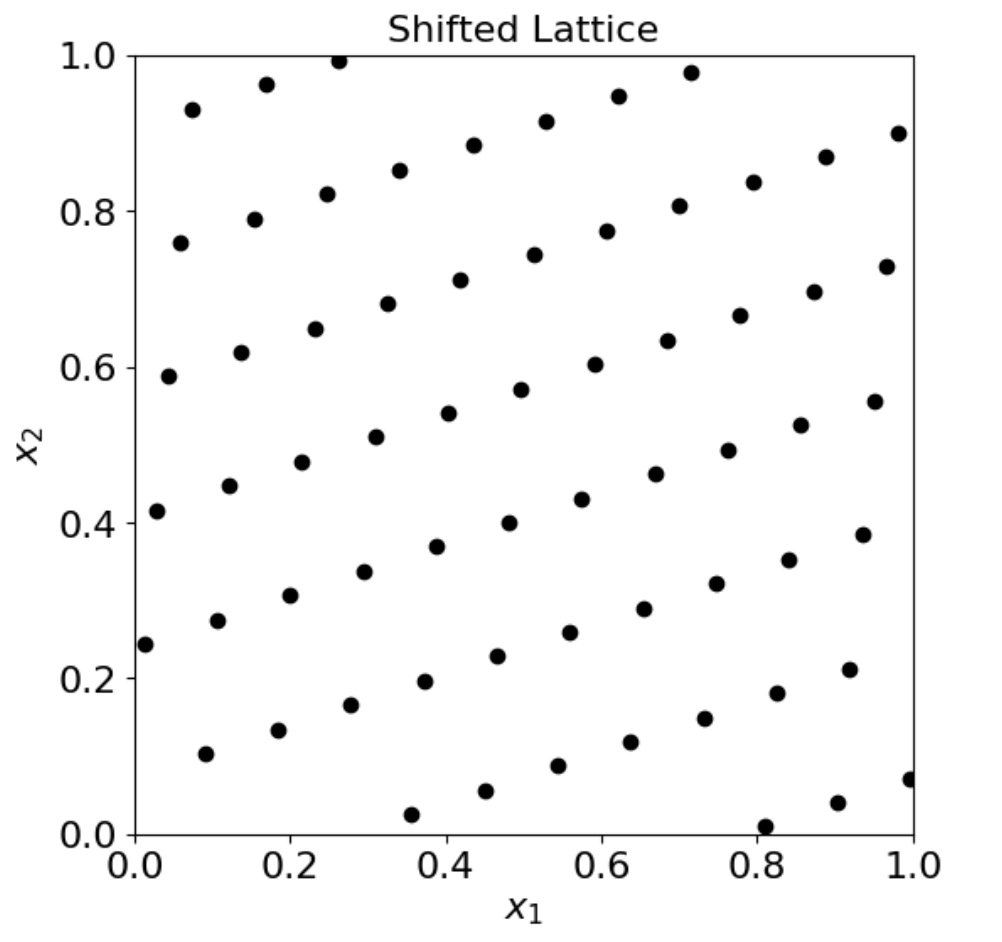
\includegraphics[width=5cm,trim={0 0 0 7.5mm},clip]{shifted-lattice}
% \caption{Two-dimensional Shifted Lattice}
% \label{fig:enter-label}
% \end{figure}

% Historically, lattice points were initially constructed as sets with fixed cardinality, $n$, and took the form
% \begin{equation} \label{eq:lat}
%     \{\vz_i = i \vh/n \bmod{\vone} : i=0,1, \ldots, n-1 \} \in [0,1)^s,
% \end{equation}
% where $\vh \in \{1, \ldots, n-1\}^s$ is the \emph{generating vector}.  A (random) shift, $\vDelta \in [0,1)^s$, is often added:
% \begin{equation} \label{eq:shlat}
%     \{\vz_i = i \vh/n + \vDelta \pmod{\vone} : i=0,1, \ldots, n-1 \} \in [0,1)^s.
% \end{equation}




Extensible lattice sequences were proposed by \cite{HicEtal00,Mai81a} and take the form
\begin{equation} \label{eq:extlat}
    \{\vz_i = \vh\phi(i)+ \vDelta \pmod{\vone} : i=0,1, \ldots \} \in [0,1)^s.
\end{equation}
where $\{\phi(\cdot)\}_{i=0}^\infty$ is the van der Corput sequence in base $b$.  In this case $\vh$ must be a generalized integer as defined in \cite[Section 2]{HicNie03a}.

The van der Corput sequence is defined as: 
\[
\phi((\cdots i_2 i_1 i_0)_b) = {}_b0.i_0 i_1 i_2 \cdots.
\]
For example, for $b=2$,
\[
\phi(6) = \phi(110_2) = {}_20.011 = \frac 38.
\]
Note that the first ${b^m}$ points of the van der Corput sequence are just equally spaced points reordered. 
\begin{equation} \label{eq:phipropone}
\{ \phi(i) : i = 0, \ldots, b^m-1 \} = \{0, b^{-m}, 2\times b^{-m}, \ldots, 1 - b^{-m} \}.
\end{equation}
Also note that
\begin{multline} \label{eq:phiproptwo}
\{ \phi(i) : i = \lambda \times b^m , \ldots, (\lambda+1)b^m-1 \} \\
= \{\phi(\lambda \times b^m) + 0, \phi(\lambda \times b^m) + b^{-m}, \ldots, \phi(\lambda \times b^m) + 1 - b^{-m} \} , \\
\lambda \in \natzero.
\end{multline}



\bibliographystyle{elsarticle-harv.bst}
\bibliography{FJH23,FJHown23}
 \end{document}